\documentclass[a4paper]{article}
\title{马尔科夫状态模型协助发现靶点的隐藏口袋}                   %———总标题
   \author{王韬 2024221120}
\usepackage{graphicx}
\usepackage{float}
\usepackage{ctex}
\usepackage{CJKutf8}
\renewcommand{\abstractname}{\textbf{\zihao{4}摘要}}
\begin{document}
	
\begin{CJK}{UTF8}{gbsn}
\CJKfamily{song}
\maketitle

\begin{center}
\tableofcontents
\end{center}

 \begin{abstract}

基于结构的药物设计(SBDD)需要预先了解特定靶点的药物结合位置,结构生物学研究中对复合物结构的解析也确实可以提供药物结合口袋的具体位置。然而,现实中的蛋白质不断运动,在运动的过程中很可能产生结构解析中无法发现的隐藏口袋。遗憾的是,大多数隐藏的口袋位点只有在解析到一个小分子可以稳定结合时才会被发现。通过课程的学习,我提出了一种方法,不使用结构生物学的方法发现隐藏的药物结合位点口袋,而是利用马尔可夫状态模型,通过马尔科夫状态间接揭示隐藏口袋。这种方法弥补了高通量筛选或者结构生物学“高成本,长周期”的缺点,为药物设计提供一种计算手段。

 \end{abstract}
\newpage


\section{马尔科夫状态模型的构建过程}
	\subsection{K-Medoids聚类}

K-Medoids算法在K-means算法的基础上衍生而来,K-Means聚类算法的目的是将分子动力学(MD)数据集划分为K个不重叠的聚类$\{C_{1},C_{2}, \cdots,  C_{k}\}$,使不同的状态与相应聚类中心(几何平均值)的距离平方和最小化。其算法可以表示为

\begin{equation}
min\sum_{i=1}^{K}\sum_{x\in C_{i}}^{} {\vert\vert x- \mu_{i} \vert\vert}^{2}
\end{equation}

其中,$x$为第$i$个聚类$C_{i}$中的MD构象,$\mu_{i}$为聚类中心。


这种方法可以对不同的MD数据进行聚类,生成“微状态”代表一部分轨迹。但这种方法的缺点在于生成的微状态并不一定是动力学过程中的一帧轨迹,原因在于K-Means方法对轨迹计算了平均值。在此,我使用K-Medoids算法进行聚类,这种方法与K-Means的区别在于K-Medoids的聚类中心选取了模拟的一帧轨迹,而非轨迹的均值,其算法可以表示为

\begin{equation}
min\sum_{i=1}^{K}\sum_{x\in C_{i}}^{} {\vert\vert x- \mathrm C(C_{i}) \vert\vert}^{2}
\end{equation}


其中,$\mathrm C(C_{i})$是作为聚类中心的构象,而非均值。


	\subsection{计算转移矩阵}
计算得到转移矩阵是构建马尔科夫过程十分重要的一个步骤,图1展示了对分子动力学轨迹构建转移矩阵的示意图。

\begin{figure}[H]
\centering
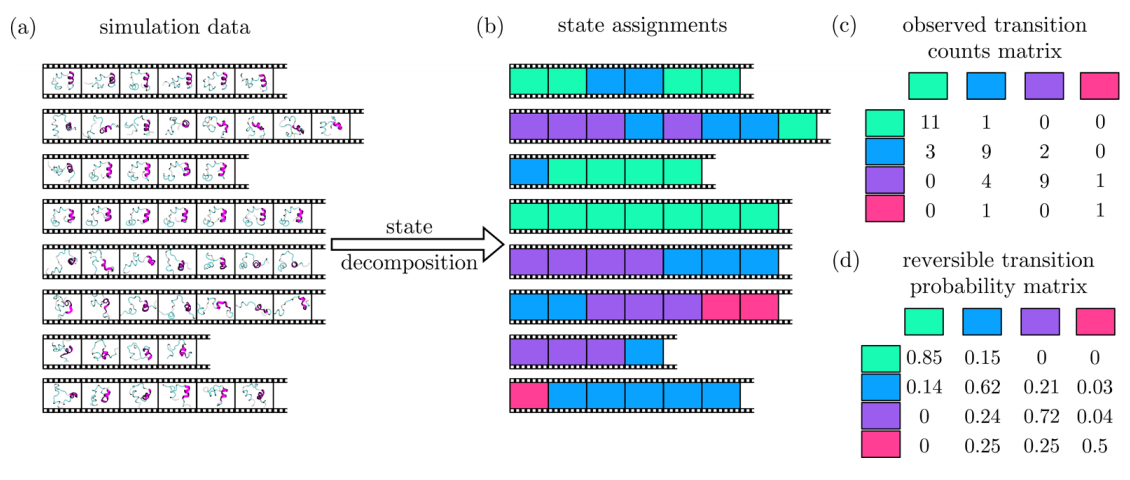
\includegraphics[scale=0.35]{trans_matrix.png}
\caption{转移矩阵示意图}
\end{figure}

K值的选取是至关重要的,在这里为了最大限度地利用模拟所生成的数据,同时也兼顾计算机的性能限制,我们使用了报道过的方法。首先对 $C_{\alpha} $和 $C_{\beta}$原子进行了均方根误差(RMSD)计算 ,随后使用 K-Medoids算法以RMSD为根据对每10 个构象进行聚类。这种方法把极其庞大的轨迹数据缩减到了原来的十分之一大小,而剩余的轨迹则被分配给这些聚类中心。

	\subsection{验证马尔科夫状态模型}

验证模型可以通过观察隐含时间尺度$t_{i}$的收敛实现,伴随着$\tau$值的不断增大,$t_{i}$应该与马尔可夫系统中的$\tau$无关。在构建转移矩阵后,我们可以得到只有一行的“特征值”,其中数值更大的特征值表示该状态衰减更慢,对应到马尔科夫过程即为更长的时间尺度。更长的时间尺度代表着更慢、可能也是更重要的过程。因此此处选取了排名前十的特征值,并以$\tau$横坐标,$t_{i}$为纵坐标作图。$t_{i}$可以使用如下公式计算


\begin{equation}
t_{i} = -\frac{\tau}{log(\lambda_{i})}
\end{equation}

其中$\lambda_{i}$为特征值, $\tau$为采样一次的时间



	\subsection{查询口袋打开情况}

为了发现隐藏口袋的开放行为,使用 Python 包 MDTraj 中实现的 Shrake–Rupley 算法计算溶剂可及表面积。对于所有蛋白质和复合物,使用 0.28 nm 的溶剂探针半径




\section{发现蛋白的隐藏位点}
	\subsection{分子动力学模拟}
		\subsubsection{蛋白选择}
		\subsubsection{模拟细节}
	\subsection{隐藏位点的寻找}




\end{CJK}
\end{document}